\documentclass[11pt]{article}
\usepackage[margin=1in]{geometry}
\usepackage{amsmath,amssymb}
\usepackage{tikz}
\usetikzlibrary{arrows.meta}
\usepackage{booktabs}
\setlength{\parindent}{0pt}
\setlength{\parskip}{6pt}

\title{Column Generation for Max Flow: Formulation and Step-by-Step Example}
\author{}
\date{}

\begin{document}
\maketitle

\section{Formulation}
\textbf{Sets and parameters}
\begin{itemize}
  \item $G=(V,A)$: directed graph with node set $V$ and arc set $A$.
  \item $s\in V$: source node; $t\in V$: sink node.
  \item $u_a\ge 0$: capacity of arc $a\in A$ (the maximum flow it can carry).
  \item $\mathcal{P}$: set of all $s$--$t$ paths in $G$. Each path $p\in\mathcal{P}$ is a set of arcs.
  \item $\mathcal{P}'\subseteq\mathcal{P}$: the subset of paths currently in the restricted master problem.
\end{itemize}

\textbf{Variables}
\begin{itemize}
  \item $f_p\ge 0$: amount of flow sent along path $p$ (primal variable).
  \item $y_a\ge 0$: dual variable of the capacity constraint of arc $a$; the price (shadow value) of one unit of capacity on $a$.
  \item $y^*_a$: the optimal dual values of the current RMP, used as arc lengths in pricing.
\end{itemize}

\textbf{Derived quantities}
\begin{itemize}
  \item $\bar c_p = 1-\sum_{a\in p}y^*_a$: reduced cost of path $p$.
  \item $x_a=\sum_{p:\,a\in p}f_p$: total flow on arc $a$ (must satisfy $x_a\le u_a$).
\end{itemize}

\textbf{Master problem (MP):}
\begin{align*}
\max\quad & \sum_{p\in\mathcal{P}} f_p\\
\text{s.t.}\quad & \sum_{p\in\mathcal{P}:\,a\in p} f_p \le u_a && \forall a\in A \quad [\text{dual } y_a\ge 0]\\
& f_p\ge 0 && \forall p\in\mathcal{P}
\end{align*}

\textbf{Restricted master problem (RMP):} the same, using only a subset $\mathcal{P}'\subseteq\mathcal{P}$.
\begin{align*}
\max\quad & \sum_{p\in\mathcal{P}'} f_p\\
\text{s.t.}\quad & \sum_{p\in\mathcal{P}':\,a\in p} f_p \le u_a && \forall a\in A \quad [\text{dual } y_a\ge 0]\\
& f_p\ge 0 && \forall p\in\mathcal{P}'
\end{align*}
The RMP has the same constraints but fewer variables. We use it because $|\mathcal{P}|$ can be exponentially large, while the RMP is small enough to solve directly.

\textbf{Dual of the MP:}
\begin{align*}
\min\quad & \sum_{a\in A} u_a y_a\\
\text{s.t.}\quad & \sum_{a\in p} y_a \ge 1 && \forall p\in\mathcal{P}\\
& y_a\ge 0 && \forall a\in A
\end{align*}
The dual value $y_a$ is the price of one unit of capacity on arc $a$ (the gain in max flow per extra unit of $u_a$).

\textbf{Pricing problem:} the reduced cost of a path is $\bar c_p = 1-\sum_{a\in p}y_a^*$. A missing path helps only if $\bar c_p>0$, so we find
\[
\min_{p\in\mathcal{P}} \sum_{a\in p} y_a^*,
\]
a shortest $s$--$t$ path with arc lengths $y^*_a$. A path costs $\sum_{a\in p}y^*_a$ in capacity and earns $1$ unit of flow.

\section{Algorithm in Words}
\begin{enumerate}
  \item Start with a small set $\mathcal{P}'$ (for example one path found by BFS).
  \item Solve the RMP and read the duals $y^*_a$.
  \item Find the shortest $s$--$t$ path using $y^*_a$ as arc lengths.
  \item If its length is less than $1$, add it to $\mathcal{P}'$ and go back to step 2.
  \item If its length is at least $1$, stop. The RMP solution is a maximum flow.
\end{enumerate}

\section{Example}
Network with nodes $s,a,b,t$:

\begin{center}
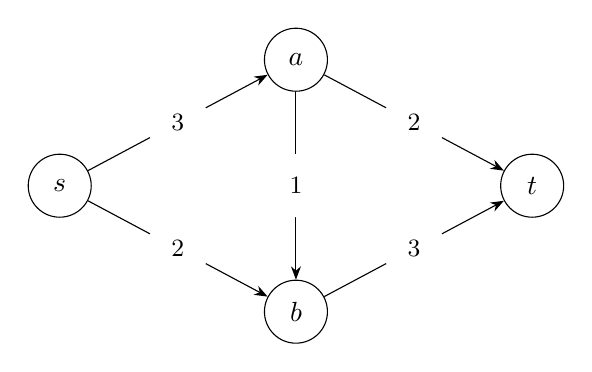
\begin{tikzpicture}[>=Stealth,
  every node/.style={circle,draw,minimum size=8mm,inner sep=0pt},
  lab/.style={draw=none,fill=white,inner sep=1pt,font=\small}]
  \node (s) at (0,0) {$s$};
  \node (a) at (3,1.6) {$a$};
  \node (b) at (3,-1.6) {$b$};
  \node (t) at (6,0) {$t$};
  \draw[->] (s) -- node[lab] {3} (a);
  \draw[->] (s) -- node[lab] {2} (b);
  \draw[->] (a) -- node[lab] {1} (b);
  \draw[->] (a) -- node[lab] {2} (t);
  \draw[->] (b) -- node[lab] {3} (t);
\end{tikzpicture}
\end{center}

Paths: $P_1=s\to a\to t$, $P_2=s\to b\to t$, $P_3=s\to a\to b\to t$. We start with $\mathcal{P}'=\{P_1\}$. Constraints are written in the order $(s,a),(s,b),(a,b),(a,t),(b,t)$.

\subsection*{Iteration 1: $\mathcal{P}'=\{P_1\}$}
\textbf{RMP:}
\begin{align*}
\max\ & f_1\\
\text{s.t.}\ & f_1\le 3 && (s,a)\\
& 0\le 2 && (s,b)\\
& 0\le 1 && (a,b)\\
& f_1\le 2 && (a,t)\\
& 0\le 3 && (b,t)
\end{align*}
\textbf{Solution:} $f_1=2$, objective $2$. Arc $(a,t)$ is full.\\
\textbf{Duals:} $y_{at}=1$, all others $0$. Dual objective: $2\cdot 1=2$ (matches).\\
\textbf{Pricing:} path lengths are $P_1=0+1=1$, $P_2=0+0=0$, $P_3=0+0+0=0$. The shortest length is $0<1$. Paths $P_2$ and $P_3$ tie; we add $P_2$.

\subsection*{Iteration 2: $\mathcal{P}'=\{P_1,P_2\}$}
\textbf{RMP:}
\begin{align*}
\max\ & f_1+f_2\\
\text{s.t.}\ & f_1\le 3 && (s,a)\\
& f_2\le 2 && (s,b)\\
& 0\le 1 && (a,b)\\
& f_1\le 2 && (a,t)\\
& f_2\le 3 && (b,t)
\end{align*}
\textbf{Solution:} $f_1=2$, $f_2=2$, objective $4$. Arcs $(s,b)$ and $(a,t)$ are full.\\
\textbf{Duals:} $y_{sb}=1$, $y_{at}=1$, others $0$. Dual objective: $2+2=4$.\\
\textbf{Pricing:} $P_1=1$, $P_2=1$, $P_3=0+0+0=0$. The shortest length is $0<1$, so add $P_3$.

\subsection*{Iteration 3: $\mathcal{P}'=\{P_1,P_2,P_3\}$}
\textbf{RMP:}
\begin{align*}
\max\ & f_1+f_2+f_3\\
\text{s.t.}\ & f_1+f_3\le 3 && (s,a)\\
& f_2\le 2 && (s,b)\\
& f_3\le 1 && (a,b)\\
& f_1\le 2 && (a,t)\\
& f_2+f_3\le 3 && (b,t)
\end{align*}
\textbf{Solution:} $f_1=2$, $f_2=2$, $f_3=1$, objective $5$. Arcs $(s,b)$, $(a,b)$, $(a,t)$ are full.\\
\textbf{Duals:} $y_{sb}=y_{ab}=y_{at}=1$, others $0$. Dual objective: $2+1+2=5$.\\
\textbf{Pricing:} $P_1=0+1=1$, $P_2=1+0=1$, $P_3=0+1+0=1$. The shortest length is $1\ge 1$, so \textbf{stop}.

\subsection*{Summary}
\begin{center}
\small
\begin{tabular}{@{}cllll@{}}
\toprule
It. & $\mathcal{P}'$ & Flows & Objective & Duals $=1$ \\
\midrule
1 & $P_1$ & $f_1=2$ & 2 & $y_{at}$ \\
2 & $P_1,P_2$ & $f_1=2,\,f_2=2$ & 4 & $y_{sb},y_{at}$ \\
3 & $P_1,P_2,P_3$ & $f_1=2,\,f_2=2,\,f_3=1$ & 5 & $y_{sb},y_{ab},y_{at}$ \\
\bottomrule
\end{tabular}
\end{center}

The maximum flow is $5$. The arcs with $y=1$, namely $(s,b)$, $(a,b)$, $(a,t)$, form the minimum cut around $\{s,a\}$ with capacity $2+1+2=5$. All three are full, and each path crosses the cut exactly once. Dual solutions are not unique here (for example $y_{sa}=y_{sb}=1$ also has cost $5$), but any of them certifies optimality.

\end{document}
